\chapter{Eliminación de palabras}

En los métodos para cuantificar la influencia de un idioma en otro, ya sea a
partir de las palabras nuevas o del uso que estas tienen en los diferentes
receptores, se ha tratado de justificar los resultados con las palabras que
intervienen en cada proceso. Sin embargo, dentro de las palabras migrantes, se encontraron errores al designar su idioma origen, errores que por el momento no se sabe ni como detectarlos ni como afectan a los resultados previos.  Una opción para detectar errores, seria al revisar cada una de las palabras por un experto en la lingüística de cada idioma, lo cual no es practico dado el tamaño de la base de datos.

Se piensa que una posible limpieza en los datos, reduciría el tamaño del corpus. Como no se cuenta con un criterio lingüístico para tal limpieza, se pueden simular reglas a partir de reducir una cantidad de palabras, y una vez hecha la reducción se obtiene el uso de un idioma en otro, para compararlo con los resultados previos. Se decidió comparar con el uso y no con las palabras nuevas, ya que en cada año hay más prestamos acumulados que préstamos nuevos (en algunos años no hay préstamos nuevos).

%Al no contar con un criterio lingüístico para una limpieza de los datos, sepiensa que la posible limpieza reducirá la cantidad de palabras, por lo que sesimularemos reglas  que reduzcan la cantidad de palabras.  Una vez hecha la reducción, 
 
%Se puede deducir que una posible limpieza en los datos reducirá la cantidad de palabras, y al no contar con un criterio lingüístico para tal limpieza, se pueden simular reglas que reduzcan la cantidad de palabras migrantes. Una vez hecha la reducción, se obtendrá el uso de un idioma en otro, para compararlo con los resultados previos. Se decidió comparar con el uso y no con las palabras nuevas, ya que en cada año hay más prestamos acumulados que préstamos nuevos (en algunos años no hay préstamos nuevos).

%Ya que no se cuenta con un criterio lingüístico para limpiar los datos, se puede utilizar la idea anterior, al simular  reglas que reduzcan la cantidad de palabras migrantes. Una vez hecha la reducción, se puede obtener el uso de un idioma en otro para compararlo con los resultados previos. Se decidió comparar con el uso y no con las palabras nuevas, ya que en cada año hay más prestamos acumulados que préstamos nuevos (en algunos años no hay palabras nuevas), además la intención de las posibles reglas, es reducir el tamaño de los conjuntos no desaparecerlos.

El proceso para reducir el corpus es el siguiente. 

\begin{enumerate}
	
	\item Se toma la lista de los préstamos acumulados de \textit{A} en \textit{B}; este corpus se denotará como \textbf{conjunto original}.
	
	\item Se escogen y descartan de forma aleatoria, a un grupo de palabras del conjunto original; este corpus  se denotará como \textbf{conjunto reducido}, mientras que el \textbf{porcentaje de reducción} $R_{p}$, es el porcentaje de palabras que se eliminaron.
	
	%de letras (desde una hasta diez), y se descartan del conjunto original a aquellas  palabras cuya primer letra sea alguna de las elegidas. El nuevo corpus se denotará como \textbf{conjunto reducido}, mientras que el \textbf{porcentaje de reducción} $R_{p}$, es el porcentaje de palabras que se eliminaron del conjunto original. 
	
	%\item Se designa un tercer corpus como \textbf{conjunto residuo}, conformado por todas las palabras eliminadas del conjunto original.  La unión del reducido con el residuo es el original. 
	
	\item En ambos conjuntos se emplea la ecuación \ref{ec.fuso} para encontrar el uso de \textit{A} en \textit{B}. %Denotando como $U_{o}$ y $U_{r}$ al uso original y al uso reducido respectivamente. 
	
\end{enumerate}

\section{Cuantificación de la similitud}

Una vez obtenidos el uso del conjunto original y el uso del conjunto reducido, lo siguiente es determinar que tan similares son los resultados.

Como en cada año el uso reducido es una porción del uso original, se define como el \textbf{factor de conversión} $F_{c}$, al promedio de dividir cada valor del uso reducido entre su correspondiente del uso original, por lo que está cantidad normalizada entre 0 y 1, es la porción entre ambos usos. 

Un factor de conversión cercano a cero, puede significar que ambos usos tengan una escala diferente a pesar de que sus respectivas graficas sean iguales. Para eliminar esta situación, se normalizaron ambos conjuntos por el valor promedio del uso de cada uno,  así los valores tanto del uso original como del uso reducido estarían alrededor de 1.  

Tras la normalización, para el año $t$ se detonan como $u_{t}$ y $r_{t}$ a los nuevos valores del uso original y del uso reducido. Se obtiene la \textbf{distancia promedio} $\left\langle D \right\rangle $, al promediar las distancias que hay entre cada valor del uso original y su correspondiente en el uso reducido: 
\begin{equation}
\left\langle D \right\rangle  = \frac{1}{N}\sum_{t=1}^{N} \left| u_{t} - r_{t} \right|  .
\label{ec.Distancia_prom}
\end{equation}
Está cantidad sera la que cuantifique que tan similares son los resultados, indicando una mayor similitud si es próxima a cero. 
%Una vez obtenidos el uso del conjunto original y el uso del conjunto reducido, lo siguiente es determinar que tan similares son los resultados. Una forma para cuantificar la similitud de ambos conjuntos, es a partir del área que comparten sus respectivas graficas; está idea se desarrollará más adelante.  

%Como en cada año el uso reducido es una porción del uso original, se define como el \textbf{factor de conversión} $F_{c}$, al promedio de dividir cada valor del uso reducido entre su correspondiente del uso original, por lo que está cantidad normalizada entre 0 y 1, es la porción entre ambos usos. 

%Un factor de conversión cercano a cero, puede significar que ambos usos tengan una escala diferente a pesar de que sus respectivas graficas sean iguales, en consecuencia el área de ellas también pueden tener una escala diferente.  Para eliminar esta situación, se normalizaron ambos conjuntos por el valor promedio del uso de cada uno,  así los valores tanto del uso original como del uso reducido estarían alrededor de 1.  

%Una vez hecha la normalización, se procedió a calcular el área compartida  $A_{c}$ de ambas graficas; esta cantidad se dividió por 109 que es el área máxima que puede haber (al ser 109 años), obteniendo así el \textbf{área de traslape}:
%\begin{equation}
%A_{T} = \frac{A_{c}}{109}.
%\label{ec.atraslape}
%\end{equation}
%Esta cantidad normalizada entre 0 y 1, indicará una mayor similitud si es próxima a uno.

\section{Características de las eliminaciones}
%$\left[0\%, 10\% \right]$, $\left( 10\%, 20\% \right]$, $\left( 20\%, 30\% \right]$, $\left( 30\%, 40\% \right]$, $\left( 40\%, 50\% \right]$, $\left( 50\%, 60\% \right]$, $\left( 20\%, 30\% \right]$, $\left( 20\%, 30\% \right]$, $\left( 20\%, 30\% \right]$,  y $\left( 40\%, 100\% \right]$. 

%Por cada intervalo se realizaron mil eliminaciones diferentes, agrupando y promediando los valores del factor de conversión y de la distancia promedio.  Ya con los promedios, será posible decir cual es el porcentaje de palabras que se puede eliminar sin que se afecten a los resultados. 


A pesar de contar con una forma de cuantificar la similitud, aun no es posible decir como se ven afectados los resultados, ya que diferentes combinaciones de palabras con las cuales hacer las eliminaciones, pueden producir distintas medidas de similitud.  No obstante, el porcentaje de reducción $R_{p}$ es útil para obtener una respuesta.

Para ello, en cada pareja de idioma origen e idioma receptor, se hicieron diez intervalos de $R_{p}$ entre el 0 y el 100, donde el primero de ellos es $\left[0\%, 10\% \right]$, el segundo $\left( 10\%, 20\% \right]$, y así sucesivamente. Por cada intervalo,  se realizaron mil eliminaciones, agrupando y promediando los valores del factor de conversión y de la distancia promedio. Las graficas de estos resultados se muestran el las figuras~\ref{fig.FC_eliminacion} y~\ref{fig.DP_eliminacion}.


\begin{figure}[h!] 
	\centering
	\begin{tabular}{cc}
		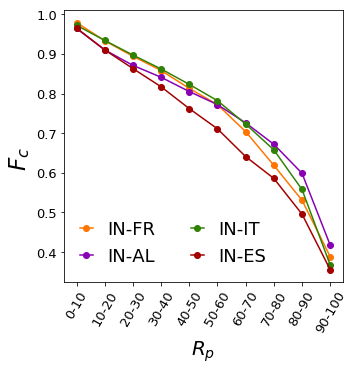
\includegraphics[width=6cm,height=6cm]{FC_EN.png} &
		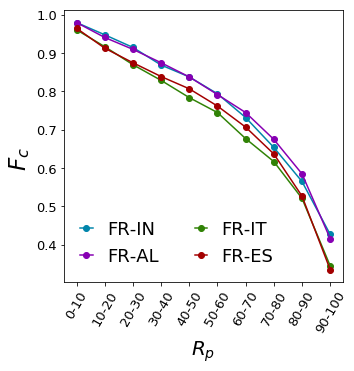
\includegraphics[width=6cm,height=6cm]{FC_FR.png} \\
		$\,\,\,\,\,\,\,\,\,\,\,\,\,\,\, \textbf{(a)}$      & 
		$\,\,\,\,\,\,\,\,\,\,\,\,\,\,\, \textbf{(b)}$     \\
	\end{tabular}
	
	\begin{tabular}{cc}
		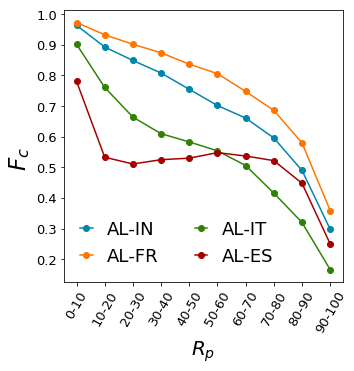
\includegraphics[width=6cm,height=6cm]{FC_GE.png} &
		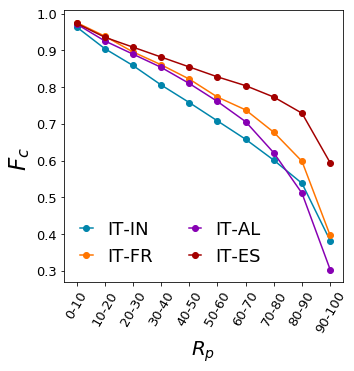
\includegraphics[width=6cm,height=6cm]{FC_IT.png} \\
		$\,\,\,\,\,\,\,\,\,\,\,\,\,\,\, \textbf{(c)}$      & $\,\,\,\,\,\,\,\,\,\,\,\,\,\,\, \textbf{(d)}$     \\
	\end{tabular}
	\begin{tabular}{c}
		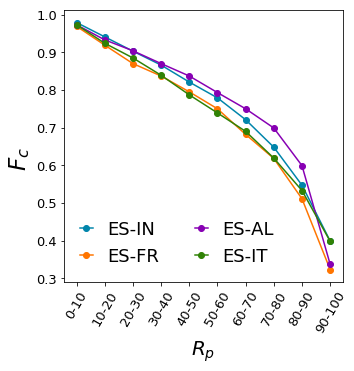
\includegraphics[width=6cm,height=6cm]{FC_SP.png} \\
		$\,\,\,\,\,\,\,\,\,\,\,\,\,\,\, \textbf{(e)}$     \\
	\end{tabular}
	\caption{Factor de conversión para distintos tamaños de reducción, en las diferentes combinaciones del inglés \textbf{(a)}, del francés \textbf{(b)}, del alemán \textbf{(c)}, del italiano \textbf{(d)} y del español \textbf{(e)}.}
	\label{fig.FC_eliminacion}
\end{figure} 


\begin{figure}[t]
	\centering
	\begin{tabular}{cc}
		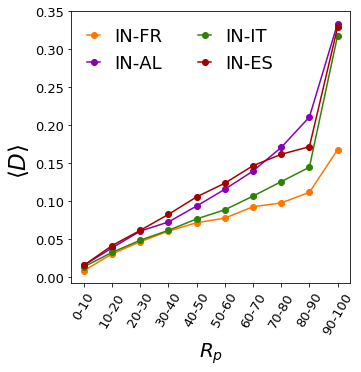
\includegraphics[width=6cm,height=6cm]{DP_EN.png} &
		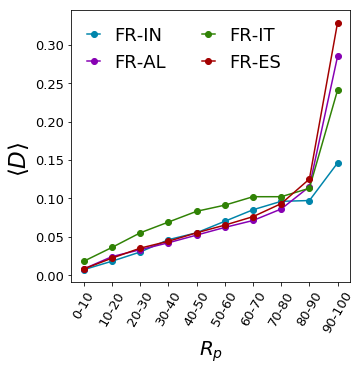
\includegraphics[width=6cm,height=6cm]{DP_FR.png} \\
		$\,\,\,\,\,\,\,\,\,\,\,\,\,\,\, \textbf{(a)}$    & 
		$\,\,\,\,\,\,\,\,\,\,\,\,\,\,\, \textbf{(b)}$ \\
	\end{tabular}
	
	\begin{tabular}{cc}
		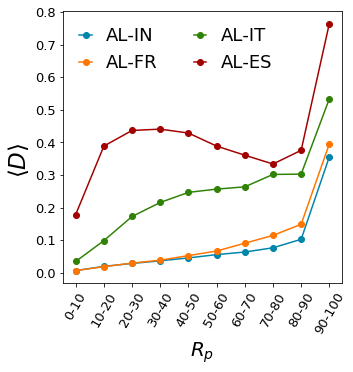
\includegraphics[width=6cm,height=6cm]{DP_GE.png} &
		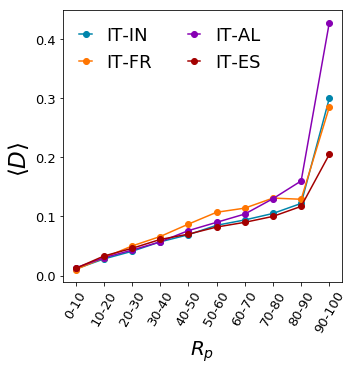
\includegraphics[width=6cm,height=6cm]{DP_IT.png} \\
		$\,\,\,\,\,\,\,\,\,\,\,\,\,\,\, \textbf{(c)}$    & 
		$\,\,\,\,\,\,\,\,\,\,\,\,\,\,\, \textbf{(d)}$    \\
	\end{tabular}
	\begin{tabular}{c}
		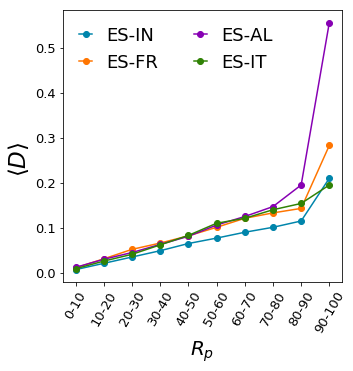
\includegraphics[width=6cm,height=6cm]{DP_SP.png} \\
		$\,\,\,\,\,\,\,\,\,\,\,\,\,\,\, \textbf{(e)}$  \\
	\end{tabular}
	\caption{Distancia promedio para distintos tamaños de reducción, en las diferentes combinaciones del inglés \textbf{(a)}, del francés \textbf{(b)}, del alemán \textbf{(c)}, del italiano \textbf{(d)} y del español \textbf{(e)}.}
	\label{fig.DP_eliminacion}
\end{figure} 


En este trabajo se considero una distancia promedio $\left\langle D \right\rangle=0.1 $, como la mínima para afirmar que los resultados no se ven afectados tras una eliminación de palabras. La tabla~\ref{tab.eliminaciones} muestra  por cada pareja de idioma origen e idioma receptor, el intervalo de $R_{p}$  y el factor de conversión $F_{c}$ donde la distancia promedio es más próxima a 0.1.

De está tabla se destaca que en 18 de las 20 parejas, se pueden eliminar más de un $40\%$ de las palabras sin verse afectados los resultados, siendo las excepciones las parejas de alemán-italiano y alemán-español.  También se puede ver una correlación entre el valor mínimo de similitud  $\left\langle D \right\rangle=0.1 $ y el factor de conversión, donde este es alrededor de $F_{c}= 0.702 \pm 0.096$.

\jmnote{aqui}


%La tabla~\ref{tab.eliminaciones} muestra por cada pareja de idioma origen e idioma receptor, el intervalo de $R_{p}$ donde el área de traslape es más próxima a 0.9 (90$\%$ de similitud), cantidad considerada (en este trabajo) como la mínima para afirmar que los resultados no se ven afectados.  Se anexa en la sección~\ref{eliminacion.completa.apendice} del Apéndice A, una segunda tabla con los valores del factor de conversión y el área de traslape de cada pareja de idiomas en cada intervalo de $R_{p}$.

%Se destaca que en 19 de las 20 parejas, se pueden eliminar alrededor del $40\%$ de las palabras yno verse afectado el uso, además en 18 parejas, con el mismo porcentaje de eliminación, la similitud es mayor al 95$\%$. 

%Por otra parte, la pareja alemán-español es la más afectada, a pesar de eliminar menos del 10$\%$ de las palabras. Una posible limpieza en esta pareja modificaría más los resultados, en consecuencia se requiere de una mayor atención al revisar a las palabras del alemán en el español. 

\begin{table}[t]
	\centering
	\begin{tabular}{cccc}
	          & \textbf{$R_{p}$} & \textbf{$F_{c}$} & \textbf{$\left\langle D \right\rangle$} \\[2pt]
		\textbf{EN-FR} & $\left( 60\%, 0\% \right]$  & 0.704 $\pm$ 0.158 &  0.093 $\pm$ 0.050 \\
		\textbf{EN-GE} & $\left( 40\%, 50\% \right]$ & 0.805 $\pm$ 0.083 &  0.094 $\pm$ 0.054 \\
		\textbf{EN-IT} & $\left( 60\%, 70\% \right]$ & 0.723 $\pm$ 0.098 &  0.107 $\pm$ 0.052 \\ 
		\textbf{EN-SP} & $\left( 40\%, 50\% \right]$ & 0.762 $\pm$ 0.142 &  0.106 $\pm$ 0.068 \\[4pt]
		
		\textbf{FR-EN} & $\left( 80\%, 90\% \right]$ & 0.565 $\pm$ 0.169 &  0.097 $\pm$ 0.055 \\
	    \textbf{FR-GE} & $\left( 70\%, 80\% \right]$ & 0.675 $\pm$ 0.015 &  0.086 $\pm$ 0.035 \\
		\textbf{FR-IT} & $\left( 60\%, 70\% \right]$ & 0.677 $\pm$ 0.170 &  0.102 $\pm$ 0.061 \\ 
		\textbf{FR-SP} & $\left( 70\%, 80\% \right]$ & 0.637 $\pm$ 0.184 &  0.093 $\pm$ 0.055 \\[4pt]
		
		\textbf{GE-EN} & $\left( 80\%, 90\% \right]$ & 0.490 $\pm$ 0.208 &  0.103 $\pm$ 0.067 \\
		\textbf{GE-FR} & $\left( 60\%, 70\% \right]$ & 0.748 $\pm$ 0.131 &  0.091 $\pm$ 0.058 \\
		\textbf{GE-IT} & $\left( 10\%, 20\% \right]$ & 0.761 $\pm$ 0.099 &  0.099 $\pm$ 0.063 \\
		\rowcolor{malo}\textbf{GE-SP} & $\left( 0\%, 10\% \right]$ & 0.781 $\pm$ 0.222 &  0.179 $\pm$ 0.210 \\
		[4pt]
		
		\textbf{IT-EN} & $\left( 60\%, 70\% \right]$ & 0.658 $\pm$ 0.160 &  0.094 $\pm$ 0.050 \\
		\textbf{IT-FR} & $\left( 50\%, 60\% \right]$ & 0.773 $\pm$ 0.131 &  0.107 $\pm$ 0.095 \\
		\textbf{IT-GE} & $\left( 50\%, 60\% \right]$ & 0.761 $\pm$ 0.114 &  0.090 $\pm$ 0.053  \\
		\rowcolor{bueno}\textbf{IT-SP} & $\left( 70\%, 80\% \right]$ & 0.773 $\pm$ 0.071 &  0.100 $\pm$ 0.040 \\[4pt]
		
		\textbf{SP-EN} & $\left( 70\%, 80\% \right]$ & 0.648 $\pm$ 0.164 &  0.101 $\pm$ 0.056 \\
		\textbf{SP-FR} & $\left( 50\%, 60\% \right]$ & 0.750 $\pm$ 0.157 &  0.101 $\pm$ 0.085 \\
		\textbf{SP-GE} & $\left( 50\%, 60\% \right]$ & 0.793 $\pm$ 0.092 &  0.106 $\pm$ 0.065 \\
		\textbf{SP-IT} & $\left( 50\%, 60\% \right]$ & 0.739 $\pm$ 0.148 &  0.110 $\pm$ 0.080 \\
		
	\end{tabular}
	\caption{Eliminaciones de cada pareja de idiomas con la mayor similitud. Entre las posibles parejas, el italiano-español \textcolor{bueno}{\rule{0.25cm}{0.25cm}} es la que mayor similitud presenta, a pesar de eliminar entre el 60$\%$ y 60$\%$  de las palabras. El alemán-español \textcolor{malo}{\rule{0.25cm}{0.25cm}} es la menor similitud pese a que en esta pareja se eliminó la menor cantidad de palabras.}
	\label{tab.eliminaciones}
\end{table}





Una conclusión que puede surgir es que la cantidad de palabras que se eliminen, influirá tanto en el factor de conversiuon como en el área de traslape. Para mostrar que esto es erróneo, se analizaran y graficaran algunos casos de eliminación, representado con un  trazo continuo al uso original, mientras que el uso reducido es una serie de puntos, también se añaden las letras con las cuales se hizo la eliminación. %así como los valores correspondientes de $R_{p}$, $F_{c}$ y $A_{T}$. 


\begin{figure}[]
	\centering
	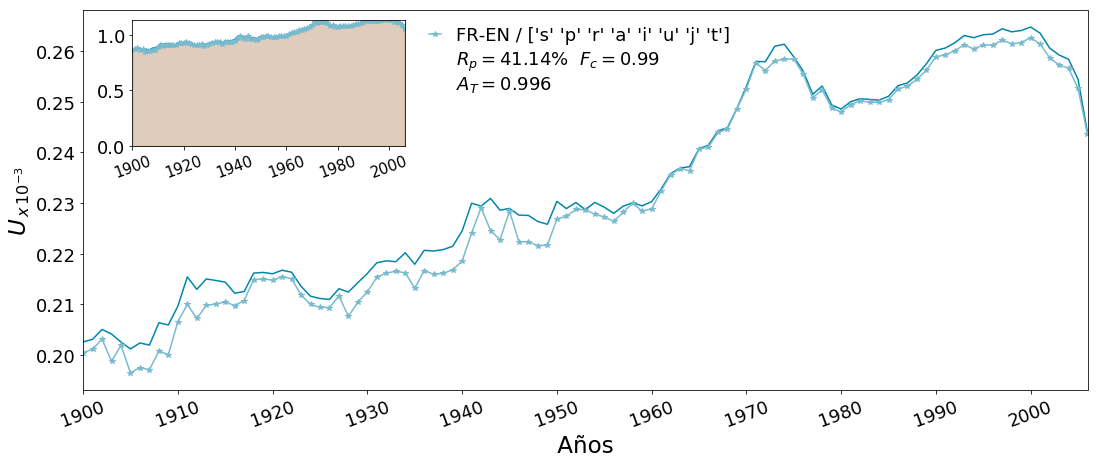
\includegraphics[scale=.375]{OM_1.png}
	\caption{Eliminación de palabras del francés en el inglés. A pesar de eliminar el 40$\%$ de las palabras del francés en el inglés, año con año el uso reducido es próximo al original y en algunos años iguales, resultando en una mayor similitud  entre ambos conjuntos al ser el área de traslape de 0.996.}
	\label{fig.OM1}
\end{figure}


\begin{figure}[]
	\centering
	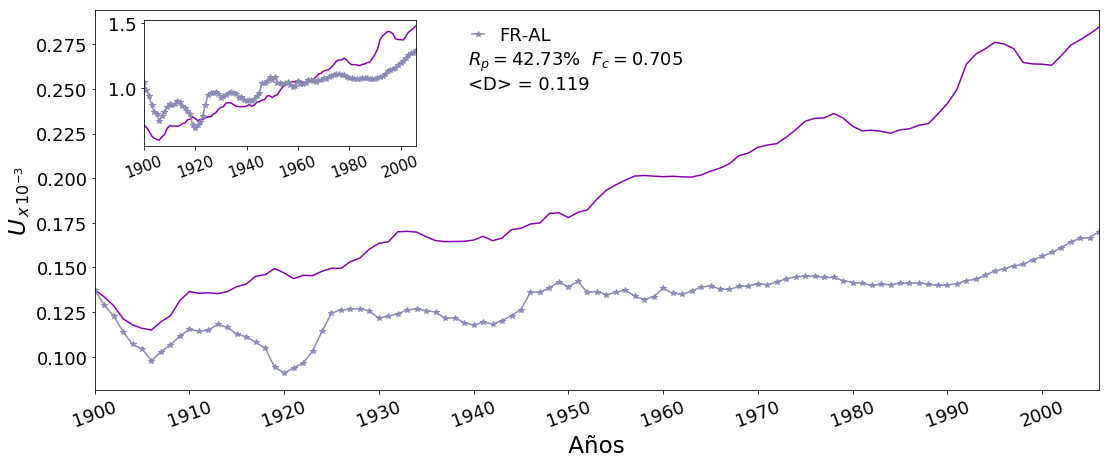
\includegraphics[scale=.375]{OM_2.png}
	\caption{Eliminación de palabras del francés en el italiano. Tras eliminar casi el 50$\%$ de las palabras del francés en el italiano, el uso en ambos conjuntos obtuvo una buena similitud de 0.946, a pesar de que cada valor del uso reducido sea en promedio la mitad de su correspondiente en el uso original.}
	\label{fig.OM2}
\end{figure}

\begin{figure}[]
	\centering
	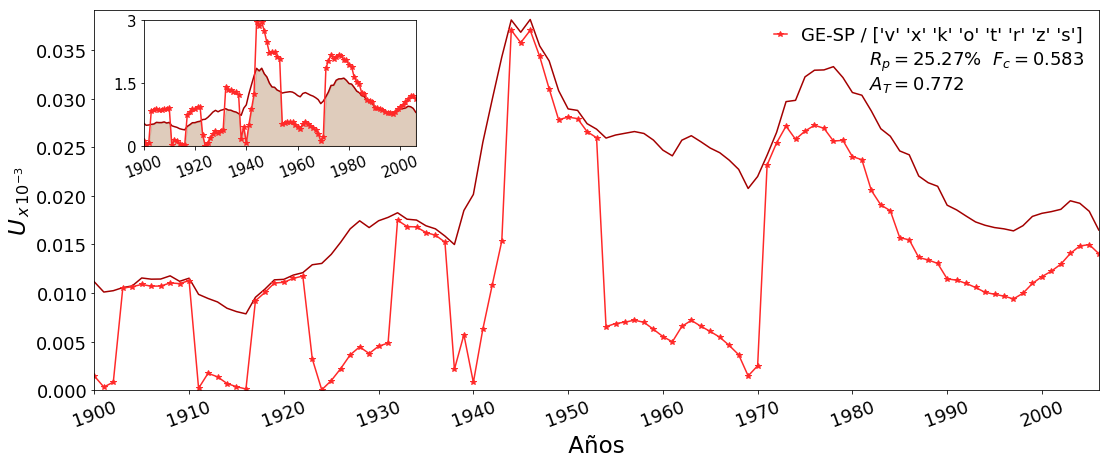
\includegraphics[scale=.375]{OM_3.png}
	\caption{Eliminación de palabras del alemán en el español. Tras eliminar el 40$\%$ de las palabras del alemán en el español, y  tener en algunos años el uso reducido y el uso original valores próximos entre si, no hay una similitud en ambos conjuntos al ser el area de traslape de 0.772}
	\label{fig.OM3}
\end{figure}


De las figuras~\ref{fig.OM1} y~\ref{fig.OM2}, se puede ver que a pesar de tener valores similares del porcentaje de reducción y del área de traslape, el factor de conversión es diferente en cada caso. Con la figura~\ref{fig.OM3}, a pesar de eliminar una cantidad menor de palabras, el área de traslape es la peor entre las tres graficas, no obstante el factor de conversión es similar al de la figura~\ref{fig.OM2}.

En conclusión, el factor de conversión es independiente de la cantidad de palabras que se eliminen (porcentaje de reducción), y ambos valores no influyen en el área de traslape.


\section{Resultados generales}

El realizar diferentes elecciones para reducir la cantidad de palabras migrantes, mostró que los posibles errores en la clasificación de los datos, no modifican (en la mayoría de los casos) los resultados obtenidos sobre el uso de un idioma en otro. Sin embargo en el caso de los préstamos nuevos, al tener mayor relevancia el significado de las palabras, una posible limpieza podría eliminar palabras de determinados campos semánticos, lo cual llevaría a perder información y a obtener resultados distintos. 

También se destaca al uso de un idioma en otro, como una propiedad común para cada pareja de idiomas, donde no tiene tanta relevancia la cantidad de palabras que conformen los préstamos acumulados,  en conjunto, todas ellas se comportarán de la misma manera. 

%El proceso de relacionar las palabras migrantes con campos semánticos y eventos históricos que justifiquen su aparición, permitió establecer un forma para cuantificar la influencia entre idiomas llamada uso. Todo este método se facilitó por la eliminación de las palabras funcionales, dejando sólo palabras de contenido, pero ¿cómo se modificaría el uso entre idiomas si se eliminaran otro tipo de palabras, sin importar si estás son de contenido?

%Para responder esta pregunta, se ha elaborado un nuevo algoritmo que reduce el conjunto de las palabras migrantes, y  obtiene nuevos valores para el uso entre idiomas.  Elegidos una pareja de idioma origen \textit{A} e idioma receptor \textit{B}, el proceso es el siguiente. 


%\jmnote{corregir "verdadero" en el parrafo}
%Si el uso en el conjunto original se toma como verdadero (ya que con el se obtuvieron los resultados del capítulo anterior), una forma de determinar que tanto cambió el uso en el conjunto reducido, es a partir del coeficiente de determinación $R^{2}$. 

%Si para un año $t$ dentro de un intervalo de tiempo $\Delta t$,  se detonan como $O_{t}$ al uso en el conjunto original y $v_{t}$ al uso en el al uso en el conjunto reducido,  mientras que $\bar{v}$ es el promedio de todos los $v_{t}$ en el intervalo, entonces el coeficiente de determinación se expresa como: 
%Para un año $t$ dentro de un intervalo de tiempo,  el uso en el conjunto original y el uso en el conjunto reducido se detonan como $O_{t}$ y $v_{t}$ respectivamente,  mientras que $\bar{v}$ es el promedio de todos los $v_{t}$ en el intervalo, entonces el coeficiente de determinación queda definido como: 
%\begin{equation}
%\label{ec.dif_uso}
%R^{2} = 1 - \sum_{t} \frac{ \left( v_{t}- O_{t} \right)^{2}  }{ \left( v_{t} - \bar{v} \right)^{2} }.
%\end{equation}
%Se empleará el concepto \textbf{conservación del uso} para aquellos idiomas cuyo uso no cambie en un intervalo de tiempo. La conservación es favorable si $R^{2}$ es próximo a 1. 
%Si la conservación no es favorable, las palabras eliminadas son las más relevantes para las migraciones de \textit{A} en \textit{B}.


%La conservación del uso y sus características no siempre serán la mismas tras una eliminación con diferentes letras, sin embargo, es posible decir con los datos de las cien mil eliminaciones, si el uso se conserva.  Para ello, se agruparon y promediaron por cada idioma origen  los valores del coeficiente de determinación, obteniendo un $\left \langle R^{2}  \right \rangle$  promedio con el cual decir de manera general, si el uso del idioma origen se conserva. 

%La tabla~\ref{tab.conservacion} muestra por cada idioma origen,  el valor de $\left \langle R^{2}  \right \rangle$ correspondiente, así como  en cuales idiomas receptores el promedio de $R^{2}$ fue mayor, y en cuales el promedio $R^{2}$ fue menor. De esta tabla se puede ver que el alemán es el idioma con los valores más bajos de $R^{2}$, donde la menor conservación se dio con el español. Los demás idiomas tienen valores aceptables con los cuales decir que su uso se conserva a pesar de las eliminaciones. 

%Como la intención de las eliminaciones es simular reglas que limpien los datos, se puede decir que los préstamos con más errores son los del alemán en el español, ya que si se hubiese tal criterio, los resultados de esta pareja serian los más afectados. En los demás idiomas no habría un cambio significativo. 

%De esta tabla se puede ver que la conservación del uso es menor, en las combinaciones donde el alemán este presente, ya sea como idioma origen o como idioma receptor. No obstante, en los demás idiomas la conservación del uso fue favorable, por lo que se puede decir que los idiomas conservan su uso, sin importar  cuales sean las palabras que conformen a las migraciones. 

%Con estos resultados se puede decir que el uso entre idiomas, no es afectado por reducir la cantidad de palabras que conforman a las migraciones,   


%\begin{table}
%	\centering
%	\begin{tabular}{cccc}
%		\textbf{} & \textbf{$\left \langle R^{2} \right \rangle$} & \textbf{$R^{2}_{max}$} & \textbf{$R^{2}_{min}$} \\
%		\textbf{inglés}   & 0.85 $\pm$ 0.14   &  IT 0.97 $\pm$ 0.01  & GE 0.77 $\pm$ 0.03  \\
%		\textbf{francés}  & 0.83 $\pm$ 0.12   &  EN 0.95 $\pm$ 0.02  & GE 0.66 $\pm$ 0.02  \\
%		\textbf{alemán}   & 0.75 $\pm$ 0.06   &  EN 0.80 $\pm$ 0.06  & SP 0.51 $\pm$ 0.33  \\
%		\textbf{italiano} & 0.87 $\pm$ 0.14   &  FR 0.93 $\pm$ 0.08  & GE 0.68 $\pm$ 0.03  \\
%		\textbf{español}  & 0.88 $\pm$ 0.05   &  IT 0.94 $\pm$ 0.06  & GE 0.71 $\pm$ 0.01                                                               
%	\end{tabular}
%	\caption{Conservación del uso de los idiomas. El español es el idioma que es menos afectado por las eliminaciones y que conserva más su uso en los demás, seguido del italiano, el inglés, el francés y por ultimo el alemán.}
%	\label{tab.conservacion}
%\end{table}



%El tratar a las migraciones de palabras como un conjunto, donde no tiene tanta relevancia las palabras que lo conforman, muestra propiedades estadísticas comunes que cumplen las parejas de idiomas. Por el momento  

   
%Individualmente. los valores de uso de una única palabra pueden ser distintos a los de otra palabra, sin embargo al tratar a todo el conjunto, el uso se comporta de la misma manera, sin importar los valores individuales de los elementos que lo conforman. 

%A pesar de haber errores en el algoritmo que clasifica tanto a los idiomas orígenes, como a sus  palabras migrantes, la conservacion del uso puede justificar que no importa si se eliminan las palabras mal clasificadas, en términos numéricos, el uso de un idioma otro va a ser el mismo.  

